%!TEX root = ../../csuthesis_main.tex

\chapter{绪论}

\section{研究背景及意义}

\subsection{研究背景}

随着深度学习的快速发展,卷积神经网络(Convolutional Neural Networks,CNN)在图像识别、目标检测、语义分割等许多任务中都展现出来了卓越的性能。在一些特定的领域任务中,部分模型的表现甚至超越了人类。但是这些网络的构建很多都依赖于经验驱动的结构堆叠,它们内部的表征机制缺乏生物解释性,与人脑视觉系统存在着显著的差距。此外,现有CNN模型在规模和计算资源上也面临挑战,随着网络层数和参数数量的增加,模型往往趋于臃肿,训练成本高昂,不利于在边缘设备上的部署;另一方面,深度网络内部表征过程缺乏透明性,其决策逻辑难以解释,被批评为“黑箱模型”,限制了其在医疗、金融等高可信度场景的推广\cite{bau2017network}。这些问题促使研究者开始思考:是否可以借助人类神经系统的结构和功能特征,引导模型设计更加轻量、解释性更强的神经网络。尽管Transformer结构的出现带来了更强的全局建模能力,但其与人类神经活动的对应性仍然有待研究\cite{ramachandram2017deep}。

神经科学研究表明,人脑的视觉处理过程具有层级结构、时间递归性和注意力调节等特征。初级视觉皮层(如V1)负责边缘、方向等低级特征编码,中层区域(如V4)整合形状和颜色等中级信息,高阶区域(如IT)则处理对象类别和语义。信息流并不是简单的单向前馈,而是在不同层之间存在大量的递归与反馈连接,构成了一个动态而复杂的加工系统。这种机制为人工视觉模型的“类脑设计”提供了理论依据\cite{dicarlo2012does}。

类脑视觉模型的提出正是为了弥补神经科学与人工智能之间的鸿沟。代表性的CORnet模型家族基于灵长类大脑腹侧通路(ventral stream)构建,具有十分清晰的区域对应关系和模块化的结构,支持神经层级对齐和可视化分析。一些研究表明,类脑视觉模型在某些特征维度上能够更好地预测神经活动模式,为理解深度网络与大脑之间的关联机制提供了有力的工具\cite{ kubilius2019brain}。

那么如何评估视觉模型与大脑的相似程度又是一个重要探讨方向。为此,Brain-Score平台的建立就显著推动了类脑建模标准化得进程\cite{schrimpf2018brain}。Brain-Score平台不仅融合了神经电生理数据与行为测试结果,还支持对视觉模型的神经预测能力进行系统打分,已经成为了当前类脑视觉模型对比实验的主流标准之一。借助该体系,研究者们得以量化模型与真实大脑在不同区域的表征一致性,从而在追求准确率之外,引入“类脑性”作为新的指标推动对模型结构的优化。

\subsection{研究目的}

类脑视觉模型的发展并非仅着眼于提高图像识别准确率,而是要探索人工神经网络与生物神经系统在表征机制方面深层次的一致性,本文研究目的在于提升模型在目标识别任务中的准确率,还期望借助神经科学分析工具Brain-Score平台,剖析模型在类脑相似性上的表现。

详细而言,本文先复现CORnet-S模型,于Tiny-ImageNet-200数据集上全面验证其在轻量结构下的识别能力与训练稳定性,接着以CORnet-Z模型为根基,引入通道注意力机制,依靠整合Squeeze-and-Excitation模块,构建结构改进版CORnet-Z+SE,以此提高其在目标识别领域的准确性,运用Brain-Score框架评估不同模型在V4和IT脑区的类脑相似性得分,并借助激活图可视化剖析不同模型对图像区域关注模式的差异。

\subsection{研究意义}

本研究有一定理论价值与实践应用意义,理论上,本文围绕类脑视觉模型CORnet-Z的结构优化问题开展,尝试把注意力机制这一近年来深度学习里的关键设计理念引入基于神经解剖结构的模型体系,此探索可深入认识人工神经网络处理视觉信息时的内部特征表达规律,且能分析其与人类大脑在层级加工机制上的异同。实践中,的结构改进方法在保持网络参数量和推理速度基本稳定的前提下,实现了分类准确率的小幅提高,这对部署在边缘计算设备、嵌入式系统或实时识别任务中的轻量化模型有一定参考作用,而且本文采用类脑相似性作为评估模型的维度之一,不再单纯将准确率当作唯一优化目标。这种多指标视角的引入拓宽了模型评价体系,还为人工智能在追求高性能时兼顾生物合理性、解释能力和系统稳定性提供了新的参考方向。

\section{国内外研究现状}

\subsection{国外研究进展}

近年来,国外在类脑视觉模型的研究取得了较为显著的进展,尤其是在深度学习与认知神经科学交叉融合的背景下,相关模型结构与评估方法不断趋于系统化和生物合理化。

在模型构建方面,Yamins等人早期提出的HMO(Hierarchical Modular Optimization)模型首次展示了深度卷积网络可以有效预测灵长类动物的IT皮层神经响应,强调了“目标驱动优化”在神经一致性建模中的核心作用\cite{yamins2014performance}。在此基础上,Kubilius等人提出的CORnet系列模型通过显式划分V1、V2、V4与IT模块,并引入时间递归结构(如CORnet-S)来模拟大脑中反馈与再入机制,是目前最具代表性的类脑网络之一\cite{kubilius2018cornet}。

在评估方法方面,Schrimpf等人建立了Brain-Score平台,为神经网络类脑程度的量化评估提供了统一框架。该平台整合了灵长类视觉皮层的电生理数据和行为响应记录,支持多种神经预测与行为一致性指标的计算,被广泛用于测试CNN、Transformer及类脑模型在不同脑区的匹配能力\cite{schrimpf2018brain}。

在注意力机制方面,许多研究开始探索将生物启发式注意力设计引入到类脑视觉模型中。Jetley等人提出通过“预测注意力热图”的方式引导卷积特征选择,实现空间级别的显著性建模\cite{jetley2018learn}。Hu等人设计的Squeeze-and-Excitation网络则通过通道注意力增强了特征表达的选择性,在多个分类任务中验证了其有效性\cite{hu2018squeeze}。Woo等人进一步提出CBAM模块,将空间注意与通道注意结合,提升了图像理解与目标检测任务中的性能表现\cite{woo2018cbam}。

值得关注的是,类脑建模的研究趋势正从静态神经对齐转向结合认知机制与任务表现的统一框架。例如Nayebi等人提出将视觉工作记忆过程建模为动态递归系统,与大脑前额叶皮层的神经活动呈现出时间一致性\cite{nayebi2018task}。Kar et al.则通过引入快速递归连接模拟目标补全与遮挡识别任务中的动态反馈,进一步提升了模型在复杂环境下的稳健性\cite{kar2019evidence}。

这些工作表明,国外学界已从单一的“神经预测”逐步转向对动态、反馈、多任务认知过程的建模尝试,推动了类脑视觉系统研究的深入发展。


\subsection{国内研究趋势与特色}

相较于国外起步较早、资源丰富,国内在类脑视觉建模方面起步相对较晚。但随着国家在人工智能领域的持续投入,类脑计算作为战略性研究方向逐渐受到广泛重视。国内多所高校与科研机构开始围绕视觉感知中的类脑机制模拟展开了系列研究,尝试将神经科学原理引入深度学习模型设计中,以提升系统的解释性与生物合理性,并形成了多条极具中国特色的研究路径。

在识别与记忆机制研究方面,曾国叙等人提出了一种基于神经相关系数(NCC)特征匹配的类脑视觉识别记忆算法,通过模拟大脑在图像识别与记忆回溯中的匹配与强化机制,实现了视觉目标的快速匹配与学习增强。这一方法在保持计算效率的同时,实现了动态记忆更新与模糊识别能力的提升,显示出良好的工程可实现性\cite{曾国叙2021ncc}。张伟等人也在相似框架下进一步优化了NCC匹配机制,增强了对小样本与遮挡图像的识别稳健性\cite{DNBC202503043}。

在视觉认知建模方面,刘建立等人从审美体验出发,提出了一种类脑计算模型架构,模拟人在面对图像、艺术作品等复杂视觉输入时的主观评价过程,探索了低级视觉特征与高级情感评价之间的耦合关系,为类脑系统中“感性-理性”协同处理提供了新方向\cite{刘建立2019视觉审美体验的类脑计算模型研究进展}。

在视觉编码机制方面,魏楚洁等人开展了多模态刺激条件下的视觉皮层反应建模工作,提出结合时序特征与空间编码规律进行类脑建模的策略,有效提升了模型在多任务切换与动态场景感知中的处理能力。研究显示,类脑模型在引入生物启发机制后,在高复杂度任务中具备更强的泛化性能\cite{1022019566.nh}。

此外,在类脑视觉与多模态融合方向,刘建伟等人提出的“类脑多模态深度学习系统”系统梳理了视觉、听觉、语言等信息通路的协同建模方式,强调跨模态对齐与注意力机制在大脑中的映射关系,为构建统一的感知认知模型提供了参考框架\cite{刘建伟2020多模态深度学习综述}。Zeng等人于2023年提出的BrainCog平台整合了大脑结构、神经元模型和大规模仿真框架,支持视觉、运动、决策等多模态任务的全流程类脑建模,是我国推动通用类脑平台标准化的重要标志之一\cite{zeng2023braincog}。


\subsection{现有研究不足}

尽管当前的类脑视觉模型在结构设计与神经预测能力方面取得了诸多成果,但整体仍处于探索阶段,存在若干关键问题有待进一步突破。

当前的类脑视觉模型在跨层级反馈机制构建上任然存在着明显的不足。生物视觉系统依赖腹侧通路与背侧通路的协同,尤其是顶叶皮层LIP区至初级视皮层V1区的反馈连接,对注意力分配至关重要。主流模型如CORnet系列仍采用单向前馈架构,仅模拟腹侧通路的时序传递,跨脑区的反馈机制还没有被有效整合\cite{kubilius2019brain}。这种简化导致模型在处理动态遮挡、视角变化等复杂任务时,缺乏生物视觉系统的特征重校准能力,与神经解剖结构存在本质差距。

现有评估体系单一。目前类脑模型的性能主要依赖Brain-Score等神经预测平台,虽然平台涵盖多个脑区的神经响应数据与行为指标,但仍存在被动对齐、维度限制等问题。例如,该平台主要集中于IT与V4区域的静态神经预测,难以涵盖动态场景、任务变化下的神经反应匹配能力。且评分结果常受到模型中间层选择的强依赖,导致类脑分数波动较大,不易跨模型比较。

现有评估体系在场景多样性和任务复杂度上显得单一。现有研究主要依赖ImageNet等静态数据集,虽然Brain-Score能够量化模型神经响应与灵长类记录的相似性,但评估场景局限于实验室标准化刺激。这难以反映模型在真实世界的动态感知能力,如光照突变、运动模糊等条件下的鲁棒性。现有指标缺乏对任务驱动型注意力机制的量化评估,无法衡量模型在主动视觉任务中的生物合理性,导致评估结果与实际应用需求脱节。

模型的可解释性依然是制约类脑模型落地的重要瓶颈。当前类脑建模多从结构对齐或性能类比角度进行验证,较少有工作从神经表征演化、神经编码稀疏性、皮层层次调节等机制角度深入分析。尤其是注意力机制引入后,其对特定神经反应模式的影响仍缺乏系统评估,模型内部激活图虽可视化程度较高,但其与神经科学中实际“感受野”或“选择性抑制”的关系尚未厘清\cite{bau2017network}。

硬件协同设计的滞后也制约了类脑视觉模型的实用化。研究多集中于算法优化,而忽视神经形态芯片、类脑传感器等硬件的开发。轻量化模型如CORnet-Z虽具实时处理潜力,但在传统GPU上能效比低。国外在神经形态芯片方向已有初步探索,例如IBM TrueNorth和Intel Loihi,但与现有模型的密集计算需求适配困难。国内在类脑计算芯片上虽然取得了突破,例如寒武纪MLU系列,但在脉冲神经网络与深度学习模型的异构融合上尚未成熟,导致算法创新难以转化为实际应用效能。


\section{本文研究内容与结构}

\subsection{本文研究内容}

本文围绕类脑视觉模型CORnet-Z展开,结合神经科学启发与模型结构改进,对其识别性能与类脑相似性进行了系统研究。主要工作如下:

\subsubsection{复现了CORnet-S和CORnet-Z模型,并在Tiny-ImageNet-200数据集上进行训练与评估,获得验证集与测试集的Top-1和Top-5准确率,用以作为基线参考,验证模型在轻量级数据集上的表现稳定性。复现过程中不仅严格对照原始参数与网络结构,还记录了模型训练过程中的收敛速度、损失变化趋势等指标。}

\subsubsection{在CORnet-Z模型基础上引入通道注意力机制(Squeeze-and-Excitation模块),构建改进模型CORnet-Z+SE,旨在增强模型对关键信息通道的选择性表达能力,并观察其对分类准确率的影响。该模块模拟了生物神经元对有意义刺激的激活调节行为,有助于模型聚焦于更具判别性的特征区域。实验中通过多次重复训练确保结果稳定,并与原始模型进行了对比验证。}

\subsubsection{利用Brain-Score评估框架,对原始CORnet-Z、引入SE模块的CORnet-Z、进一步引入CBAM注意力机制与VOneBlock的结构改进模型进行神经一致性评估,分析各模型在V4与IT层的类脑得分变化趋势,并与ResNet-18、AlexNet等典型模型进行横向比较。}

\subsubsection{基于激活图可视化方法,提取并对比CORnet-Z模型与改进后添加了SE模块的模型在不同层级的激活图,观察注意力机制对特征图关注区域的调节作用,并初步探讨模型内部的可解释性变化。通过对图像区域响应热力图的对比分析,进一步揭示不同模型对目标信息处理路径的变化,辅助解释类脑相似性得分差异的成因。}

通过上述工作,本文试图探讨注意力机制在类脑视觉模型中的作用效果,以及结构改动对识别准确率与神经一致性之间可能存在的权衡关系。

\subsection{本文结构安排}

全文总共被划分成五个章节,各章的具体内容是这样的:

第一章是绪论部分,讲述了本研究的背景以及意义,对国内外在类脑视觉模型领域的研究现状做了综述,并结合了当前CNN面临的模型庞大、缺乏解释性等挑战,明确提出以神经解剖对齐为核心的研究方向,最后简单说明了一下论文的整体结构。

第二章主要梳理类脑视觉模型构建所依靠的理论基础,囊括人类视觉系统的层级结构、神经解剖对其机制、反馈机制以及注意力调节原理,着重分析CORnet模型家族的设计思路、选择CORnet-Z作为改进基线的动因以及Brain-Score等评估标准的构成方式。

第三章基于通道注意力机制的CORnet-Z模型优化 以模型构建与优化为核心,首先复现了CORnet-S和CORnet-Z两种类脑模型,在Tiny-ImageNet数据集上进行训练与和析,为后续改进提供性能参考。之后,引入SE通道注意力机制并嵌入CORnet-Z的多个模块,构建改进模型CORnet-Z+SE,分析模块结构、集成方式以及训练表现,评估其在准确率与收敛速度方面的改进效果。

第四章主要介绍类脑模型的评估方法以及结果分析,重点运用Brain-Score框架和MajajHong2015公开神经数据集对各版本模型在V4与IT脑区的神经预测能力进行定量对比,凭借对多个指标得分的统计分析,并通过激活图可视化方法,探索模型结构变化与类脑相似性之间的关系。

第五章是总结与展望,总结本文的主要研究工作和阶段性成果,讨论当前研究中的不足之处,并对未来在结构改进、任务拓展与神经评估方法等研究方向做了初步展望。

\begin{figure}[hbt]
	\centering
	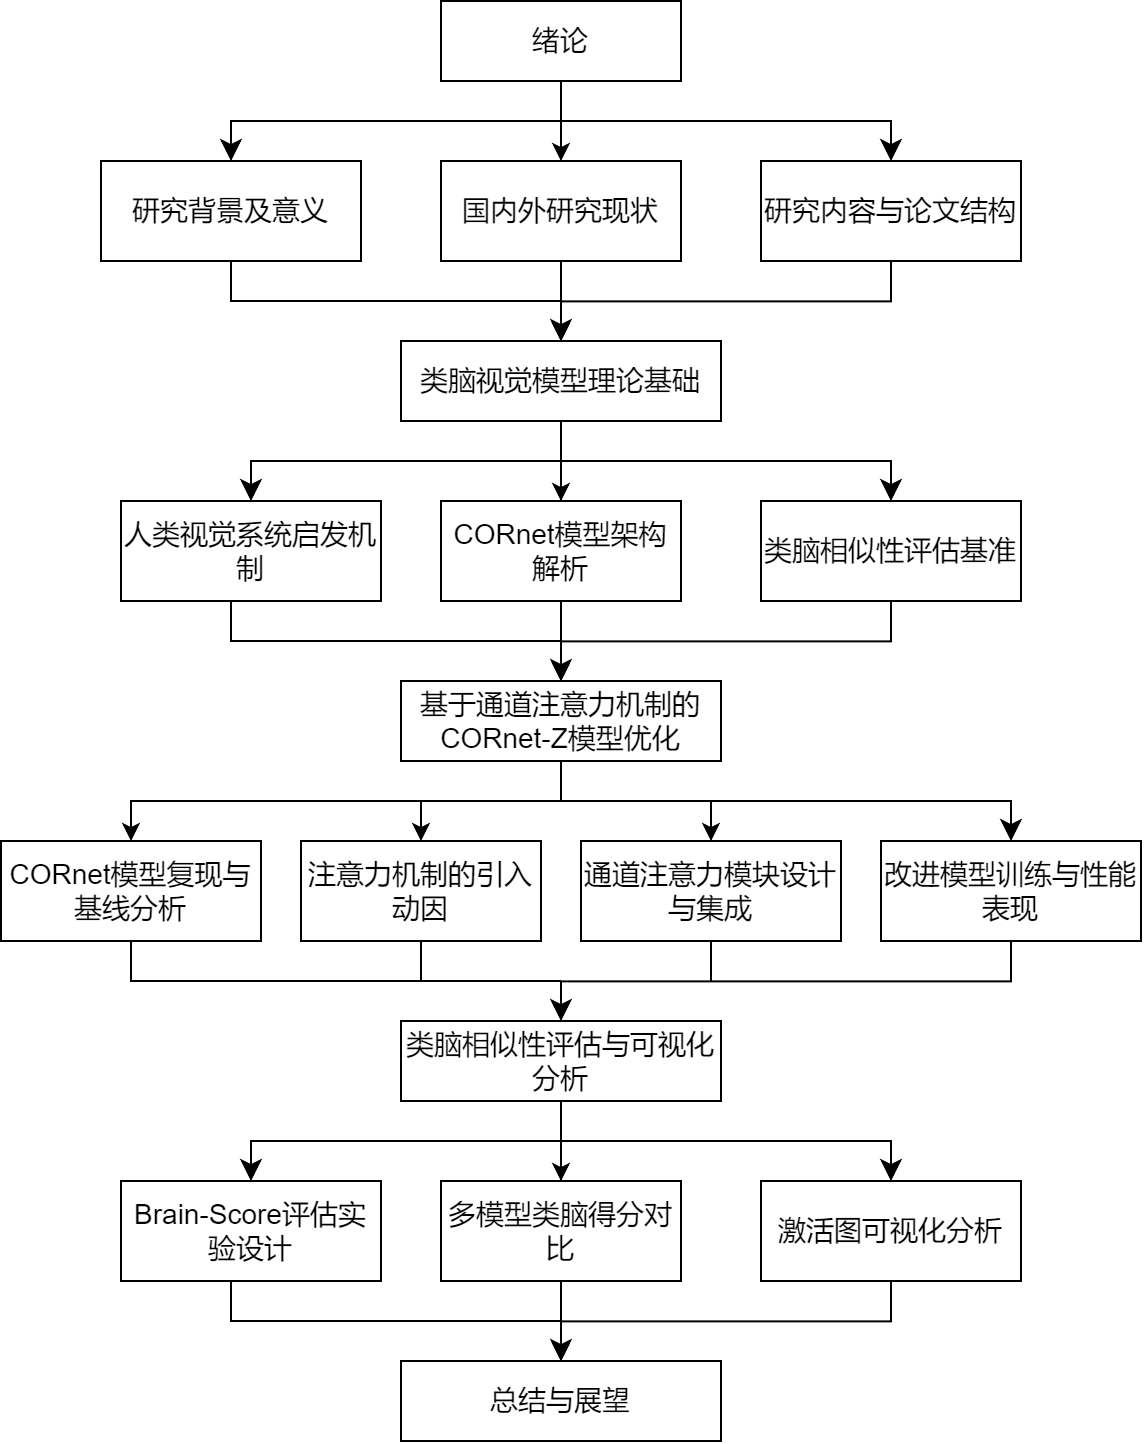
\includegraphics[width=0.8\linewidth]{论文框架.png}
	\caption{论文结构框架}
	\label{f.lunwenkuangjia}
\end{figure}
